% !TeX root = ../main.tex
\chapter{Broadband photon pair generation}\label{chap:7}

Back to the classical nonlinear optics theory, the solution to nonlinear coupling equations requires the initial power at ether signal or idler mode, which is called seed light in the laser terminology. However, in quantum optics theory, all the cavity modes behave intrinsic vacuum fluctuation at a quantity of half $ \hbar \omega $. Generally, even without light fed, the quantum fluctuation leads to photon emission at the single photon levels. 

Once the single photon flux exceeds cavity threshold, the extracavity photon can be detected. To note, this kind of excitation is indistinguishable because the signal and idler photons are emitted simultaneously as a result of quantum mechanics, rather than signal photon stimulates idler photon and vice versa. 
In the language of quantum states, the state created intracavity contains both signal and idler photons. The wave packet is different from the normal single photon one. Further theoretical research \cite{Scully1997} explained the squeezed nature of four wave mixing photon pairs, which is one of the exclusive properties of frequency entangled photon pairs.

In general, the photon pair or mode pair defined in our context refers to cavity modes are excited collectively under the phase matching condition. 
All the pairs are at a superposition of probability amplitude.
Thus, under the weak coherent approximation, only two correlated photons exist in the wave packet, but the basis depends on allowed mode pair.
Coincidence counting technology can be used to verify such correlation. As to generation band, it agrees with the classical phase matching condition.

\section{Methods}

Using the dispersion extraction method in \autoref{chap:5}, zero dispersion wavelength can be located easily among the measured band. In our experiments, optical communication band, especially C band is concentrated on, because enormous fiber optical components, like in-line filters are available in this range.

Illustrated in \autoref{fig:bibpf}, the setup of mode-resolvable singular photon pair generation first adopts a tunable laser as the pump source, whose display tunability is 0.1 pm and able to be tuned via external voltage input. The laser output is pumped into ring resonators using the fiber launching system.% and the output power is measured with the power meter. 

A simple transmission scanning is then perform to select polarization mode.
For high \textit{Q}-factor devices, the transmission of TE and TM modes are separated in a distance of tens of pm. Thus, as either of the resonance vanished by rotating the polarization controller, the fiber launches the particular polarization mode in the bus waveguide. For low \textit{Q}-factor cavities, since the TE and TM are degenerate in the spectrum, the method of polarization alignment is as same as the one using the InGaAs infrared camera.

Beyond the polarization selection, the pump wavelength should also be aligned to the cavity resonance. The on-resonance or off-resonance can be determined as the output power displays maximal distinction ratio. In our experiment, the pump peak around 1550 nm, usually presents at least 10 dB extinction before and after on-resonance.

Next, the output light are splitted 50\si{\percent} by 50\si{\percent} into signal and idler channels, indicating half of generated photons are lost. The two channels are sequentially filtered through two sets of band pass filters (Haphit Inc.). The pass band in the first set is 1540$\pm$4 nm and 1560$\pm$4 nm, respectively. The second set of band pass filters are tunable (WL Photonics Inc.) whose 3dB bandwidth is 0.12 nm. Since the free spectra range (FSR) in our device is much larger, the tunable band pass filter is adequate to select single mode at both channels.

Finally, each channel are detected by superconducting single photon detectors (SNSPD, SCONTEL) which are specific for infrared range. Since the SNSPD is polarization-sensitive, another two polarization controllers (not shown in \autoref{fig:bibpf}) are used to achieve maximal single photon counting during each measurement. At last, the time controller (ID Quantique, ID900) collects and records the counting time tag in the 100 ps resolution. Here, coincidence counting can be triggered directly or calculated later by data processing. The common coincidence window used in our experiments is 1 ns.

\begin{figure}
	\centering
	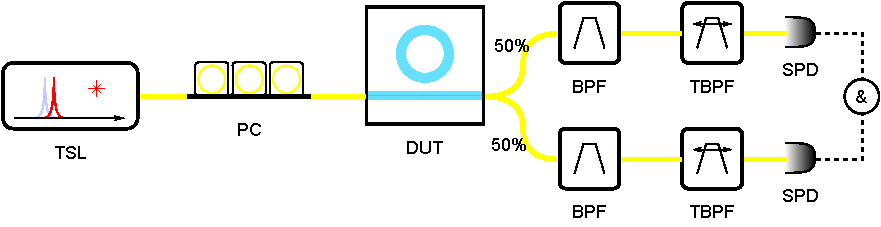
\includegraphics[width=1\linewidth]{imgs/biBPF.pdf}
%	\includesvg[width=.9\textwidth]{setup/biBPF}
	\mycaption{Setup of mode-resolvable singular photon pair generation}{TSL, tunable semiconductor laser. PC, optical fiber polarization controller. DUT, device under test. BPF, band pass filter. TBPF, tunable band pass filter. SPD, single photon detector.}
	\label{fig:bibpf}
\end{figure}

\bigskip
\noindent\textbf{Coincidence counting}

In quantum optics, coincidence counting is usually used to examine the non-locality of singular wave-particle. In our case, the photons which are splitted into two channels A and B yields the count per second (cps) $N_\mathrm{A}$ and $ N_\mathrm{B} $. Define the coincidence windows $t$, 1 ns commonly, and coincidence count (CC) is the number of two photon trigger events within this small time window, equivalent to the photon pair generation rate effectively. The accidental counting (ACC) is defined as $ N_\mathrm{A} N_\mathrm{B} t $, alike to the background noise of counting system. Thus accidental-coincidence ratio (CAR) is defined as (CC-ACC)/ACC to reduce the noise effects.

It is worth to mention that in our research, the main topic is photon pair generation rather than photon state manipulation, in result numerous band-pass filters are exploited to realize mode-resolvable single photon counting. It does not contradict with distinguishability nature of frequency correlated photon pairs.


\section{Low power photon pair generation}
In this chapter, considering the mode spacing and \textit{Q}-factors, LIGENTEC Group 2 Device 1 is mainly employed to perform photon generation, whose spectrum is presented in \autoref{fig:ligentec_gp1}. This device has FSR of 150 GHz and shows anomalous dispersion around 1550 nm given in \autoref{fig:dint_comp}.

\begin{figure}
	\centering
	\includesvg[width=4in]{ligentec/ligentec_gp1}
	\mycaption{Transmission, quality factors and FSR of LIGENTEC Group 2 Device 1 employed in this chapter}{$ D_2 $ = 1.47 MHz and \textit{Q}-factor is around \num{2.5d5} in the filter band.}
	\label{fig:ligentec_gp1}
\end{figure}

\subsection{Single mode photon flux}

With the pump power set as 100 \si{\micro\watt} and central wavelength at 1550.64 nm, the result of photon flux at both signal and idler bands versus relative relative mode index is presented in \autoref{fig:flux1}. According to the 3dB bandwidth of band pass filters (BPF), the accessible relative mode index corresponds 7-14. To achieve higher photon counting, the central wavelength of tunable band pass filters (TBPF) is tuned carefully in the step of 0.01 nm.

In the result, there is trend that both signal and idler photon fluxes decreases as the mode index increases. It can be explained that phase mismatch of farther modes is greater than closer ones. The difference between signal and idler bands origins from the asymmetry of phase matching condition and filter spectral shape. As the input power is set as 100 \si{\micro\watt}, the estimated photon generation rate is around \num{d3} cps/\si{\micro\watt} per mode.

\begin{figure}
	\centering
	\includesvg[width=5in]{mode_depen/flux_1}
	\mycaption{Photon flux with 100 \si{\micro\watt} pump power}{The pump power set as 100 \si{\micro\watt} and central pump wavelength is at 1550.64 nm. Selected modes is from 1536 nm to 1544 nm for idler band and 1556 nm to 1564 nm for signal band.}
	\label{fig:flux1}
\end{figure}


\subsection{Coincidence counts of singular mode pair}

In coincidence counts are measured in a 1ns coincidence window and in each mode, the time delay is set from -200 to 200 ps. The \autoref{fig:mode_cf} shows the result of coincidence counts and CAR. In the mode pair 9, single photon pair generation rate is 1500 per second, equals to \num{1.5d4} cps per mW, which is the highest rate observed at this input power level among all the samples.

As the mode number increases, coincidence counts varies roughly but in the CAR graph, such a trend is not obvious. This is due to the band pass filters used in our setup is not flat-top on the transmission spectrum. In conclusion, even several frequency-dependent optical components used in our setup, by calculating the coincidence-accidental ratio, the photon pair generation can be evaluated successfully.

\begin{figure}
	\centering
	\includesvg[width=5in]{mode_depen/mode_cf}
	\mycaption{Coincidence count and CAR at filtered modes}{Pump power is 100 \si{\micro\watt}. Coincidence window is 1 ns.}
	\label{fig:mode_cf}
\end{figure}

\section{Pump power dependence}

Since spontaneous four wave mixing originates from Kerr nonlinearity, in classical nonlinear optics, converted power is linearly dependent on pump power. To confirm this relation in quantum scale, it is necessary to study both power dependence of photon flux and coincidence counts.

To amplify the pump power, a erbium-doped fiber amplifier (EDFA) is cascaded after the tunable laser. By increasing the output power, the power intracavity can exceed 500 mW. 
The mode passed through is fixed at $ \mu=9 $, corresponding to $\lambda_\mathrm{i}$ = 1540.28 nm and $\lambda_\mathrm{s}$ = 1558.79 nm. During each cavity resonance alignment, the extinction ratio is kept around 10 dB. 
The result of photo flux is given in \autoref{fig:pwflux}. It is apparent that there is a continual growth of photon flux in both signal and idler modes. 

\begin{figure}
	\centering
	\includesvg[width=3in]{pw_depen/pw_flux}
	\mycaption{Power dependence of photon fluxes during photon pair generation}{The input power is the power measured at the input port.}
	\label{fig:pwflux}
\end{figure}

\begin{figure}
	\centering
	\includesvg[width=5in]{pw_depen/pw_cc_acc}
	\mycaption{Power dependence of coincidence count and coincidence-accidental count ratio during photon pair generation}{The input power is the power measured at the input port.}
	\label{fig:pwcar}
\end{figure}

Furthermore, the coincidence counting result is shown in \autoref{fig:pwcar}(a) where both maximal coincidence counts and background accidental coincidence counts increase with the pump power. While from CAR provided in \autoref{fig:pwcar}(b), higher input power leads to a significant decline. This can explained by the background noise arising from the Raman effect in optical fibers \cite{Engin2012, Sugiura2019}
. As the nonlinearity of optical fibers is much weaker than silicon nitride device, in the high input power regime, it becomes obvious and contributes to the single photon count and decreases the coincidence count rate.

\section{Joint spectral intensity}

Since the spontaneous four wave mixing occurs simultaneously at each mode pair, the state generated in a broadband is equivalent to the intensity superposition all over the signal and idler bands. To clarify the quantum state characteristics in this view, usually the joint spectral filed or intensity is estimated to evaluate the frequency correlation \cites{Helt2010,Vernon2015b}. For example, compared with the $ N $ mode correlation measurement mentioned above, the two-party joint spectral intensity requires the coincidence measurement on the element in the whole $ N^2 $ hilbert space.

On the other hand, much of recent research concerning soliton generation discussed the thermal instability in the nonlinear ring resonators \cites{Guo2017a,Herr2012}. 
To realize long time stable measurement, an auxiliary photon diode is added to monitor off-resonance situation illustrated in \autoref{fig:pid}. Using digital proportional–integral–derivative (PID) controller, which is deployed by a LabVIEW program, the tunable laser wavelength is tuned dynamically by the external voltage input. In this way, the extinction ratio of on-resonance is kept at a stable level as soon as possible. In addition, to increase the accessible mode number, the first set of BPFs in \autoref{fig:bibpf} is replaced by a notch filter (OE Land Inc.). The pump power used here is 24.5 mW. This work is assisted by Kenta Sugiura.

\begin{figure}
	\centering
	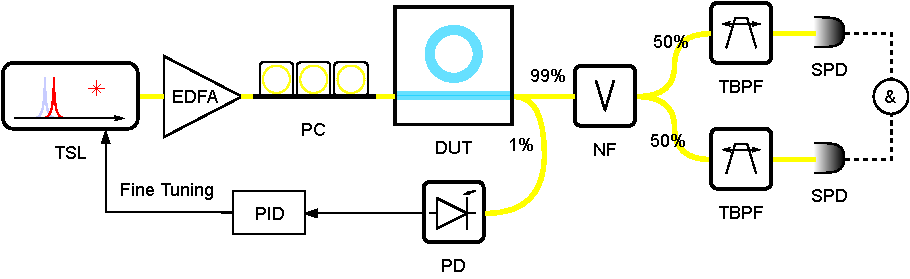
\includegraphics[width=1\linewidth]{imgs/pid.pdf}
	\mycaption{Setup of long-time stable photon pair generation}{TSL, tunable semiconductor laser. PC, optical fiber polarization controller. DUT, device under test. NF, notch filter. TBPF, tunable band pass filter. SPD, single photon detector.PD, photodiode. PID, digital proportional–integral–derivative.}
	\label{fig:pid}
\end{figure}

%\autoref{fig:jsi} presents the final results of intermodal coincidence counts, accidental coincidence counts and their ratio, CAR. 
During our measurement, the coincidence count is first scanned along the diagonal term of joint spectral intensity map to locate the central wavelength of tunable band pass filters when photon flux in \autoref{fig:flux2} is measured. In \autoref{fig:jsi}(a), CC characterizes the peak at mode 13. This agrees with the result of photon flux. More obviously, both photon flux and CC suffer from the notch filter, whose 3dB cut bandwidth is larger the single FSR and not symmetric at signal and idler bands. After the diagonal scanning, the off-diagonal terms are then selected mode-by-mode. The grid-like distribution in ACC map, \autoref{fig:jsi}(b) indicates the variation of measurement.
As a result, the CAR presented in \autoref{fig:jsi}(c) stands out no obvious off-diagonal fluctuation and features the frequency correlation in 46 mode pairs, corresponding a 106 nm ( 1499 nm - 1605 nm) span.

\begin{figure}
	\centering
	\includesvg[width=5in]{jsi/flux_2}
	\mycaption{Photon flux at 24.5 \si{\micro\watt} pump power of LIGENTEC Group 2 Device 1}{The mode near the central wavelength is effected by the notch filter.}
	\label{fig:flux2}
\end{figure}

\begin{figure}
	\centering
	\includesvg[width=6in]{jsi/jsi_map}
	\mycaption{Coincidence count, accidental coincidence count and coincidence-accidental count ratio used to evaluated joint spectral intensity}{The pump is 24.5 mW and the mode span corresponds to the range from 1499 nm to 1605 nm.}
	\label{fig:jsi}
\end{figure}

\bigskip
In this chapter, the frequency entangled photon pair is successfully generated using a high \textit{Q}-factor anomalous dispersive silicon nitride ring cavity. The power dependence is studied and the mode-resolvable setup is performed thus a maximal 46 pairs of entangled photons is observed spontaneously, at 24.5 mW pump power.

%\section{Summary}
